\section{Radio Controller}
The radio controller, used to manoeuvre the vehicle, is a Radiolink AT9 9 channel
2.4GHz control system. The controller supports the provided Radiolink R9D
9 channel, 2.4 GHz DSSS (Direct-sequence spread spectrum) receiver.

\subsection{Steering}
The Layout of the buttons on the controller can be seen in
\cref{fig:controller_front} and \cref{fig:controller_back}, for the front and
back of the controller respectively. In \cref{fig:controller_front} the
\textit{Elevator/Rudder stick} is used to control the speed of propellers
driving the vehicle forward. The propellers will not move when the stick is in the
lowest position in the figure, and will have max speed when the stick is in the
top most position in the figure. Note that the stick should be put in the
lowest position when the electronics of the vehicle is powered on. Be careful to not run the propulsion motors too hard, as they tend to overheat.

The \textit{Throttle/Aileron Stick} is used to control the air rudders. Moving
the stick to the right will turn the vehicle to the right and moving it to the
left will turn it left.

The stick on the back of the controller, the \textit{VRC SW} stick in
\cref{fig:controller_back} is used to control the rotational speed of the RBRs.
If the stick is in the bottom most position the RBRs will not rotate. By moving
the stick upwards the speed will increase until the stick is in the top
position. Be sure to move the stick slowly when accelerating the RBRs, otherwise the top speed might not be reached. 

\begin{figure}[h]
   \centering
   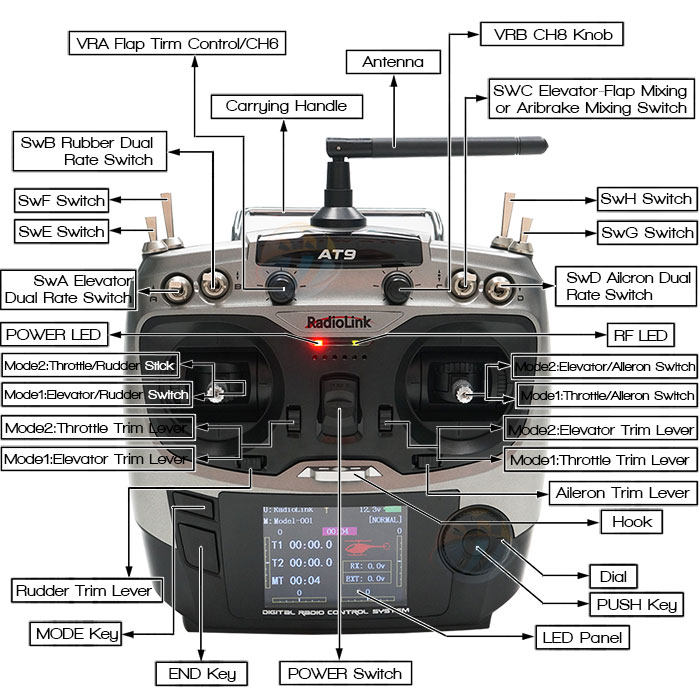
\includegraphics[width=.75\textwidth]{controller_front}
   \caption{The front of the radio controller, together with its buttons.}
   \label{fig:controller_front}
\end{figure}

\begin{figure}[h]
   \centering
   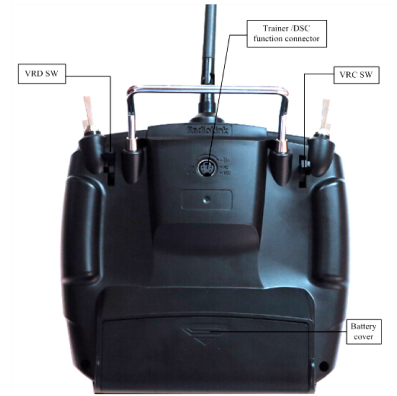
\includegraphics[width=.75\textwidth]{controller_back}
   \caption{The back of the radio controller, together with its buttons.}
   \label{fig:controller_back}
\end{figure}

\subsection{Settings}
When it comes to the controller settings, the base settings of the Helicopter type was used, which can be found under \textit{Model sel.} in the basic
menu of the controller. The basic menu is found by holding in the \textit{mode}
button.

Some settings however were changed to be able to maneuver the vehicle
more easily. The first of these setting tweaks were to put channel 1-3 from
normal to reversed, in order to get the buttons to behave in a way better
suited for a vehicle. This is done in \textit{reverse}, which can be found in the
Basic menu. In order to get the \textit{VrC SW} button on the back of the
controller, used to control the rotational speed of the RBRs (see
\cref{fig:controller_back} for button layout), one has to go into
\textit{AUX-CH} in the basic menu and choose which channel  one want to couple
it with. Then select \textit{VrC} on that channel. We chose to use channel 5,
but any other channel can be used as well.
